\documentclass[11pt, a4paper]{article}
\usepackage[utf8]{inputenc}
\usepackage[T1]{fontenc}
\usepackage[british]{babel}
\usepackage{amsmath}
\usepackage{amssymb}
\usepackage{graphicx}
\usepackage[textwidth=16cm, textheight=25cm]{geometry}
\newcommand{\ind}{\mathbb{I}}
\newcommand{\eqdef}{\mathrel{\stackrel{\text{def}}=}}
\newcommand{\ddd}{\mathrm{d}}

\author{Gautam \textsc{Tripathi}}
\title{Convolutions of kernels}

\pagestyle{empty}

\begin{document}
	
\maketitle
\thispagestyle{empty}


Let $k^*(x) \eqdef \int_{\mathbb{R}} k(u) k(x-u)\,\ddd u$.

1. $k$ is uniform $[-1,1]$ kernel. If $k(u)\eqdef \frac12\ind(|u|<1)$, then
\[
k^*(x) = \frac14 (2-|x|), \quad -2\le x \le 2.
\]

2. $k$ is triangular kernel on $[-1,1]$, i.\,e. $k(u) \eqdef (1-|u|) \ind(|u|\le 1)$. Then
\[
k^*(x) = \begin{cases}
\frac16 (4 - 6 |x|^2+ 3 |x|^3 ), & 0\le |x| \le 1,  \\
\frac16 (8 - 12|x| + 6|x|^2 - |x|^3), & 1 < |x| \le 2. \\
\end{cases}
\]

3. $k$ is Epanechnikov kernel on $[-1,1]$, i.\,e. $k(u) = \frac34 (1-u^2) \ind(|u|\le1)$. Then
\[
k^*(x) = \frac{3}{160} (32 - 40 |x|^2 + 20 |x|^3 - |x|^5), \quad -2 \le x \le 2.
\]

4. $k$ is quartic kernel on $[-1,1]$, i.\,e. $k(u)\eqdef \frac{15}{16} (1-u^2)^2 \ind(|u|<1)$. Then
\[
k^*(x) = \frac{225}{256} \left(\frac{256}{315} -\frac{128}{105} |x|^2 + \frac{16}{15} |x|^4 - \frac{8}{15} |x|^5+ \frac{4}{105} |x|^7 - \frac{1}{630} |x|^9 \right), \quad  -2 \le x \le 2.
\]

\vfill

\centering
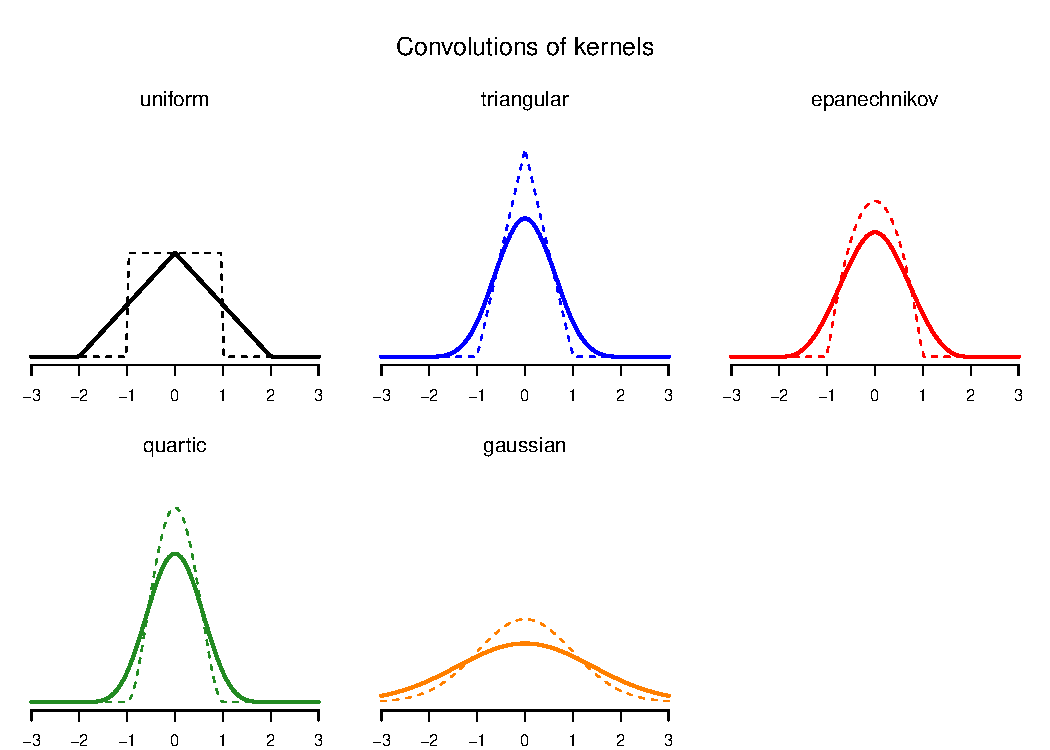
\includegraphics[width=0.8\textwidth]{output/12-convolutions.pdf}


\end{document}

